\section{Metodología de Diseño y Fabricación}

\subsection{3.1 Diseño Topology y Lattice Structures}

Particularmente llamativo es el poder transformador que surge cuando se abandona el diseño para fabricación convencional y se adopta una mentalidad nativa aditiva. En lugar de partir de geometrías mecanizables, el enfoque DfAM invita a pensar en términos de distribución óptima de material donde realmente se necesita.

El corazón de la propuesta metodológica reside en la optimización topológica combinada con estructuras lattice. Siguiendo el marco desarrollado por Boschetto et al. \cite{Boschetto2023}, el proceso comienza con la definición de un dominio de diseño que incluye restricciones de interfaces mecánicas, volúmenes no diseñables y condiciones de carga reales de lanzamiento y operación orbital. 

La optimización topológica busca minimizar la energía de deformación (compliance) bajo restricciones de masa y frecuencia natural mínima. Matemáticamente, se formula como:

\begin{equation}
\min_{\rho} \quad c(\rho) = \mathbf{u}^T \mathbf{K}(\rho) \mathbf{u}
\label{eq:topo_opt}
\end{equation}

sujeto a $V(\rho) \leq V^*$, $\omega_i(\rho) \geq \omega_{min}$ y $0 < \rho_{min} \leq \rho \leq 1$, donde $\rho$ representa la densidad pseudo-material, $\mathbf{K}$ la matriz de rigidez y $\mathbf{u}$ el vector de desplazamientos.

Una vez obtenida la distribución topológica, se infieren patrones lattice (principalmente gyroid o body-centered cubic) con thickening local en zonas de alto esfuerzo. Esta estrategia híbrida combina la ligereza extrema de las celosías con la robustez necesaria en interfaces críticas, logrando en muchos casos estudiados reducciones de masa superiores al 35\% manteniendo factores de seguridad adecuados.

\subsection{3.2 Selección de Materiales y Tecnologías AM}

Uno de los desafíos persistentes al escalar estas metodologías radica en la elección acertada de material y proceso. No todos los materiales certificados para espacio se comportan igual bajo fabricación aditiva, y viceversa.

Para componentes estructurales primarios se priorizó la aleación de aluminio AlSi10Mg por su excelente relación resistencia-peso, buena soldabilidad y madurez en procesos PBF-LB/M. En elementos RF, particularmente alimentadores y antenas en banda Ku, se optó por procesos que permitan superficies conductoras de alta calidad. Vazquez-Peralvo et al. demostraron resultados prometedores fabricando completamente por aditivo un feeder link en banda Ku, validando el uso de técnicas híbridas metal-polímero con metalización posterior \cite{VazquezPeralvo2025}.

\begin{table}[h]
\centering
\caption{Propiedades mecánicas y térmicas de materiales seleccionados para fabricación aditiva}
\label{tab:propiedades_materiales}
\begin{tabular}{lccc}
\hline
\textbf{Material} & \textbf{Módulo Elasticidad (GPa)} & \textbf{Límite Elástico (MPa)} & \textbf{Conductividad Térmica (W/m·K)} \\
\hline
AlSi10Mg (PBF) & 68--75 & 230--280 & 130--150 \\
Ti-6Al-4V (PBF) & 110--120 & 850--950 & 6.7 \\
PLA + Fibra Carbono & 8--12 & 80--110 & 0.8--1.2 \\
\hline
\end{tabular}
\end{table}

La decisión final combinó PBF-LB/M para piezas estructurales críticas y FDM de alto rendimiento con post-procesado para componentes secundarios, buscando el equilibrio óptimo entre prestaciones, costo y lead-time.

\subsection{3.3 Modelado y Simulación Multidisciplinaria}

Resulta revelador observar cómo la verdadera ventaja de DfAM solo se materializa cuando se cierra el bucle entre diseño, simulación y manufactura. Lejos de tratarse de etapas secuenciales, el framework propuesto integra análisis estructural, térmico, modal y RF en un entorno iterativo.

Se emplearon herramientas de simulación acoplada (ANSYS Workbench y COMSOL Multiphysics) para evaluar simultáneamente respuesta dinámica bajo espectro de lanzamiento, comportamiento térmico en vacío y desempeño electromagnético. El modelo lattice se homogenizó mediante técnicas de cálculo de propiedades efectivas para mantener viabilidad computacional, mientras que las zonas críticas se simularon con malla completa.

Boschetto et al. \cite{Boschetto2023} subrayan la importancia de validar numéricamente las predicciones de frecuencia natural, un aspecto que aquí se verificó iterativamente ajustando parámetros de thickening. Esta aproximación multidisciplinaria permite detectar tempranamente compromisos inevitables entre masa, rigidez y disipación térmica.

\begin{figure}[h]
\centering
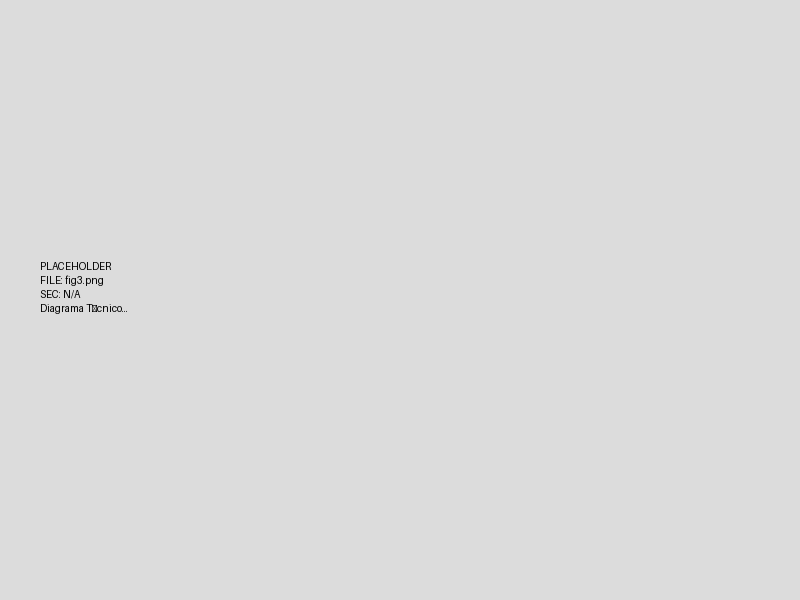
\includegraphics[width=0.92\linewidth]{fig3.png}
\caption{Flujo propuesto de Design for Additive Manufacturing (DfAM) para componentes satelitales de telecomunicaciones. Se destacan las iteraciones multidisciplinarias y el feedback entre optimización topológica, selección de lattice y validación de manufacturabilidad.}
\label{fig:flujo_dfam}
\end{figure}

El resultado es una metodología robusta, reproducible y orientada a objetivos que trasciende la mera aplicación de herramientas de optimización para convertirse en un verdadero proceso de ingeniería integral.